\subsection{Grundprinzip}

Wenn Elektronen durch einen Leiter fließen, erzeugen sie einen Strom, der in einer Spule ein Magnetfeld aufbaut (Siehe \referenz{subsec:MFeldSpule}). Beim Aufbau dieses Magnetfeldes ändert sich dieses, logischerweise. Diese Änderung erzeugt allerdings in der selben Spule auch wieder eine Induktion, die sogenannte Selbstinduktion, deren Strom gemäß der Lenz'schen Regel (Siehe \referenz{sec:Lenz}) entgegengesetzt der eigentlichen Stromrichtung gerichtet ist.

Dies führt dazu, dass der Stromfluss "gebremst" wird.

\subsection{Verhalten beim Unterbrechen eines Stromkreises}
%Cue for review (Induziert man einen Strom oder eine Spannung?)

Wenn in einem Stromkreis eine Spule mit Strom durchflossen wurde und sich in ihr das Magnetfeld vollständig aufgebaut hat, wird bei einer abrupten Unterbrechung des Stromkreises das Magnetfeld zusammenbrechen und aufgrund dieser starken Änderung ($\Delta t$ ist sehr klein) eine hohe, entgegengesetzt gepolte Spannung induziert.

\begin{figure}
	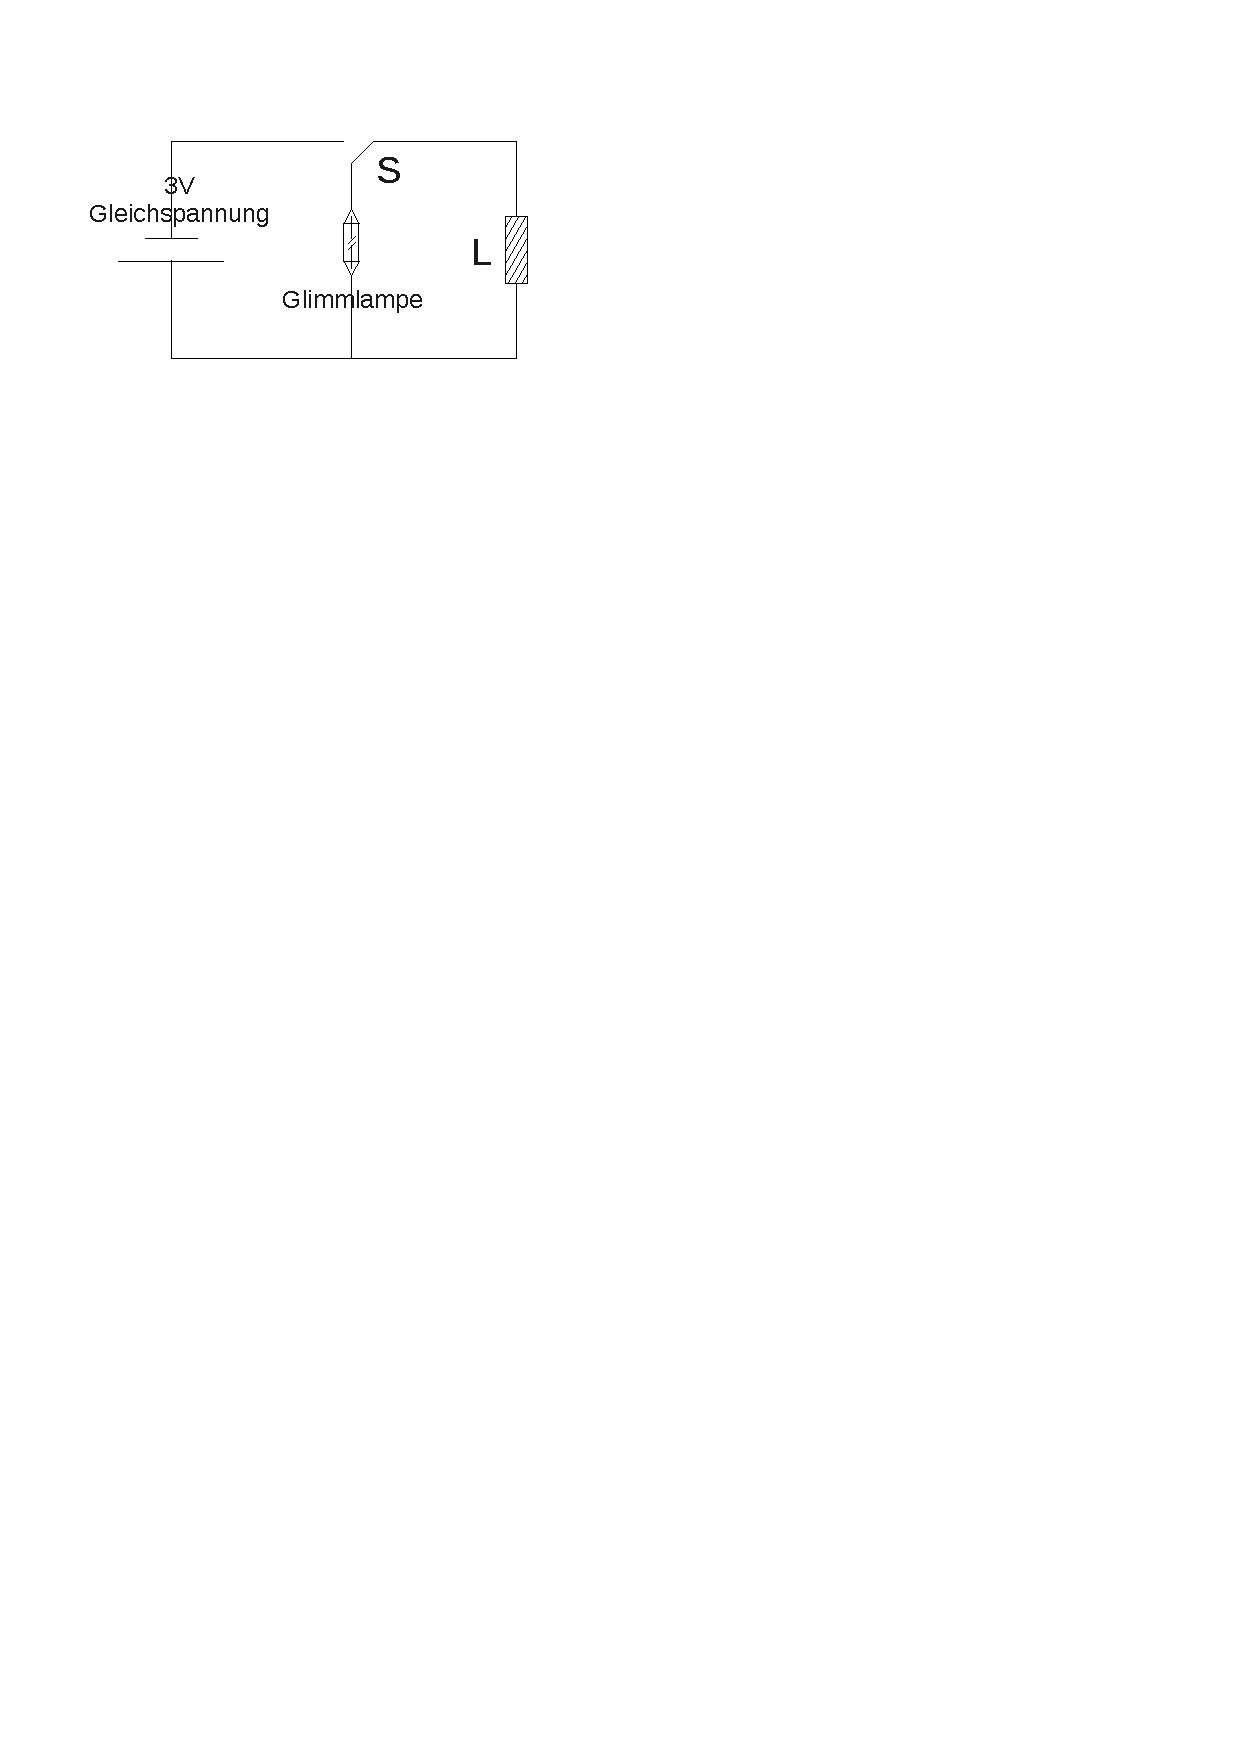
\includegraphics[width=\textwidth]{SelbstinduktionGlimmlampe}
	\caption{Möglicher Schaltkreis mit einer Glimmlampe, die eine hohe Auslösespannung benötigt. \textbf{S} ist ein Schalter der Wahlweise die Gleichspannungsquelle oder die Glimmlampe mit der Spule verbindet.}
	\label{fig:SchaltkreisGlimmlampe}
\end{figure}

Dies lässt sich mit einer parallel zur Spule geschalteten Glimmlampe veranschaulichen, die eine Auslösespannung von circa 60 - 70 Volt besitzt. Sie wird beim Ausschalten des Stromkreises leuchten, auch wenn die Spannung bisher nur wenige Volt betrug.\footnote{"SelbstinduktionGlimmlampeSChaltkreis" von Till Blaha - Eigenes Werk. Lizenziert unter Gemeinfrei}